\documentclass[tikz]{standalone}
\usepackage{fontspec}
\renewcommand*{\familydefault}{\sfdefault}
\usepackage{standalone}
\usetikzlibrary{decorations.pathreplacing}
\usetikzlibrary{arrows.meta, decorations.pathreplacing, shapes.geometric}
\usetikzlibrary{bayesnet}

\begin{document}
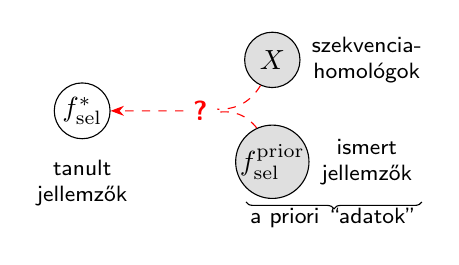
\begin{tikzpicture}
% Define nodes
\path (0,0)
node[latent] (U1) {\(f_\mathrm{sel}^\ast\)}
to
(15:2.5 cm)
node[obs] (X) {\(X\)}
to
(-15:2.5 cm)
node[obs, inner sep=0] (U2) {\(f^{\mathrm{prior}}_\mathrm{sel}\)}
(U1) +(0:1.5 cm) node[font=\bfseries, red] (fusion) {?}
;

\path[font=\footnotesize]
(X) +(0:1.2 cm) node[align=center] (seq) {szekvencia-\\homológok}
(U2) +(0:1.2 cm) node[align=center] (feat) {ismert\\jellemzők}
(U1) +(-90:0.5 cm) node[anchor=north, align=center] {tanult\\jellemzők}
;
\draw[decorate, decoration={brace, mirror, raise=5 pt}] (U2.south west) --
node[label=below:{a priori ``adatok''}] {} (U2.south west -| feat.south east);

\draw[dashed, red, -Stealth]
(X) to[bend left] (fusion)
(U2) to[bend right] (fusion)
(fusion) -- (U1)
;

\end{tikzpicture}

\end{document}


